\chapter{光电倍增管的性能测试与筛选}
\label{ch:pmt_test}

\section{PMT批量测试平台}
\label{sec:pmt_test:testbench}
\emph{为什么需要特质的批量测试平台}

\subsection{功能与特点}

\begin{figure}[htb]
	\centering
	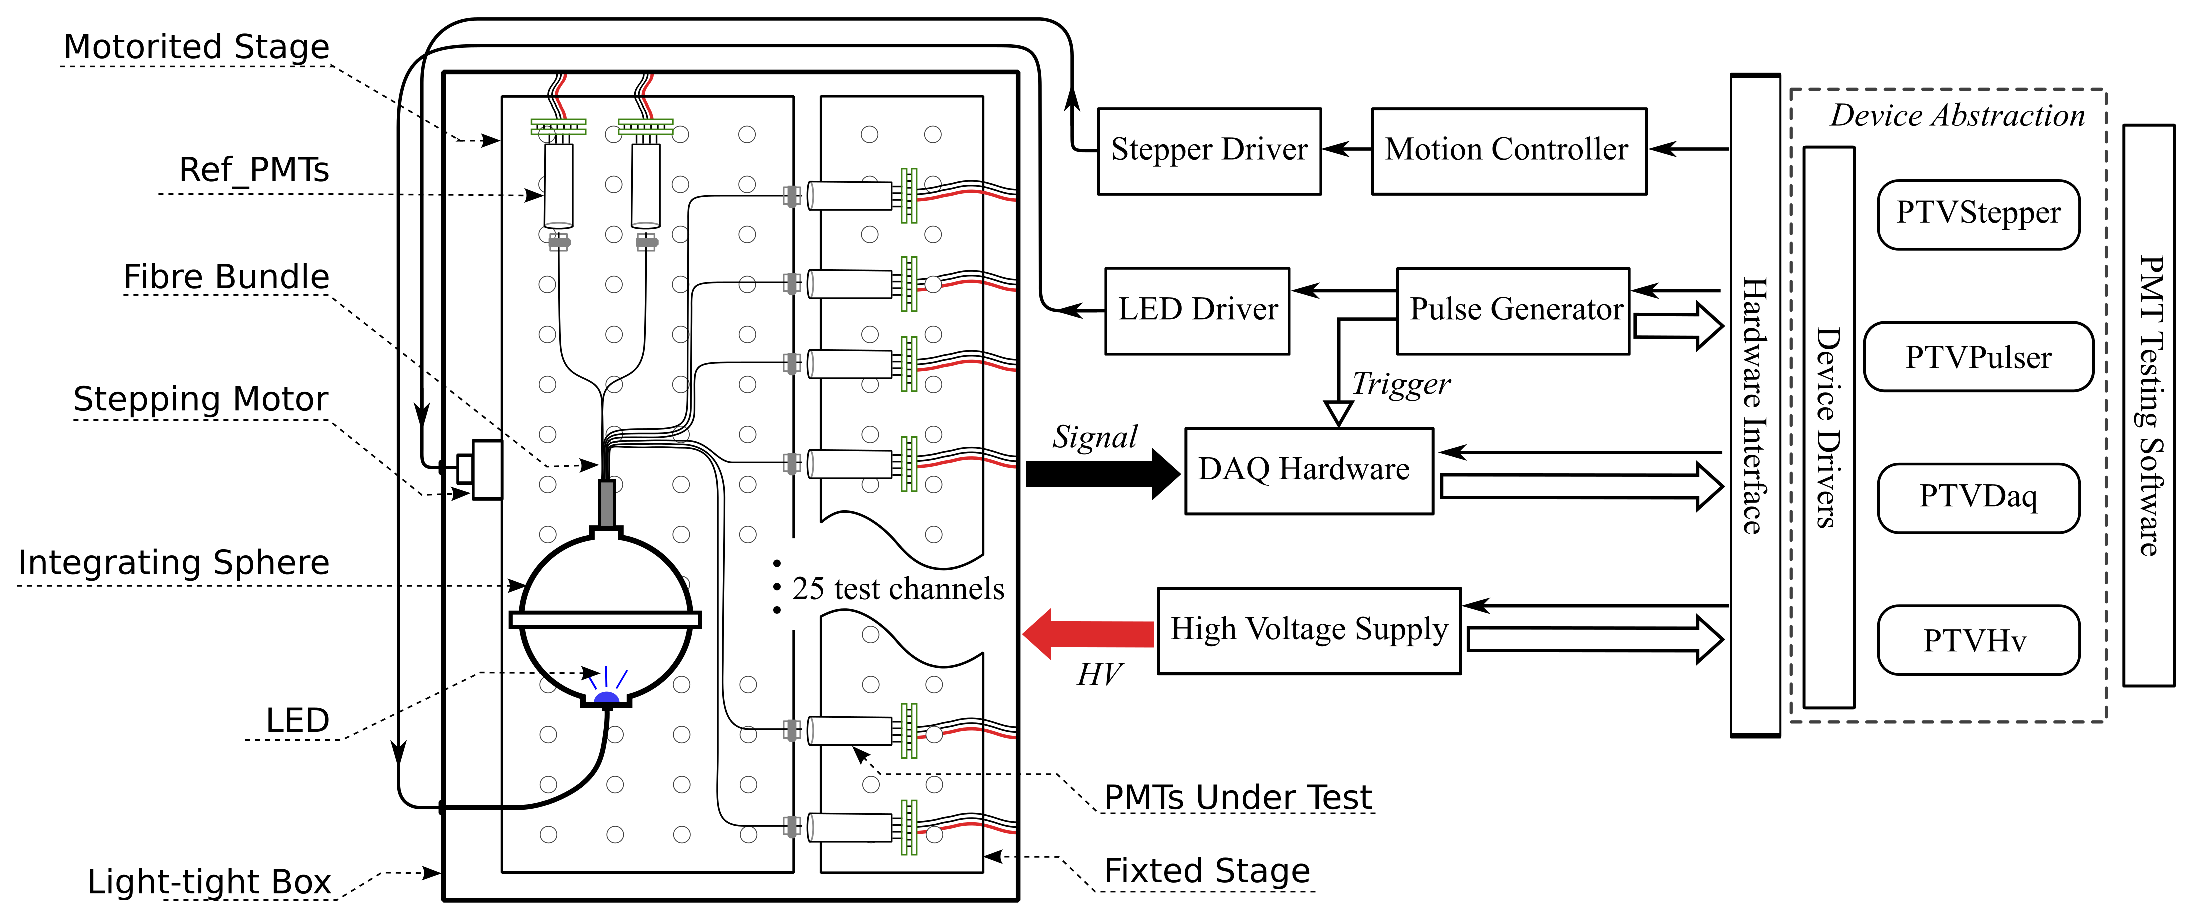
\includegraphics[width=\textwidth]{chap/pmt_test/fig/testbench_schematic.eps}
	\caption{PMT批量测试平台的原理框图}
	\label{fig:pmt_test:testbench_schematic}
\end{figure}

\subsection{硬件结构与组成}
% 总述硬件结构,之后依次介绍各组件以及相关测试结果。

% 主体平台
\begin{figure}[htbp]
	\centering
	\subfloat[][铝合金暗箱]{
		\label{fig:pmt_test:blackbox}
		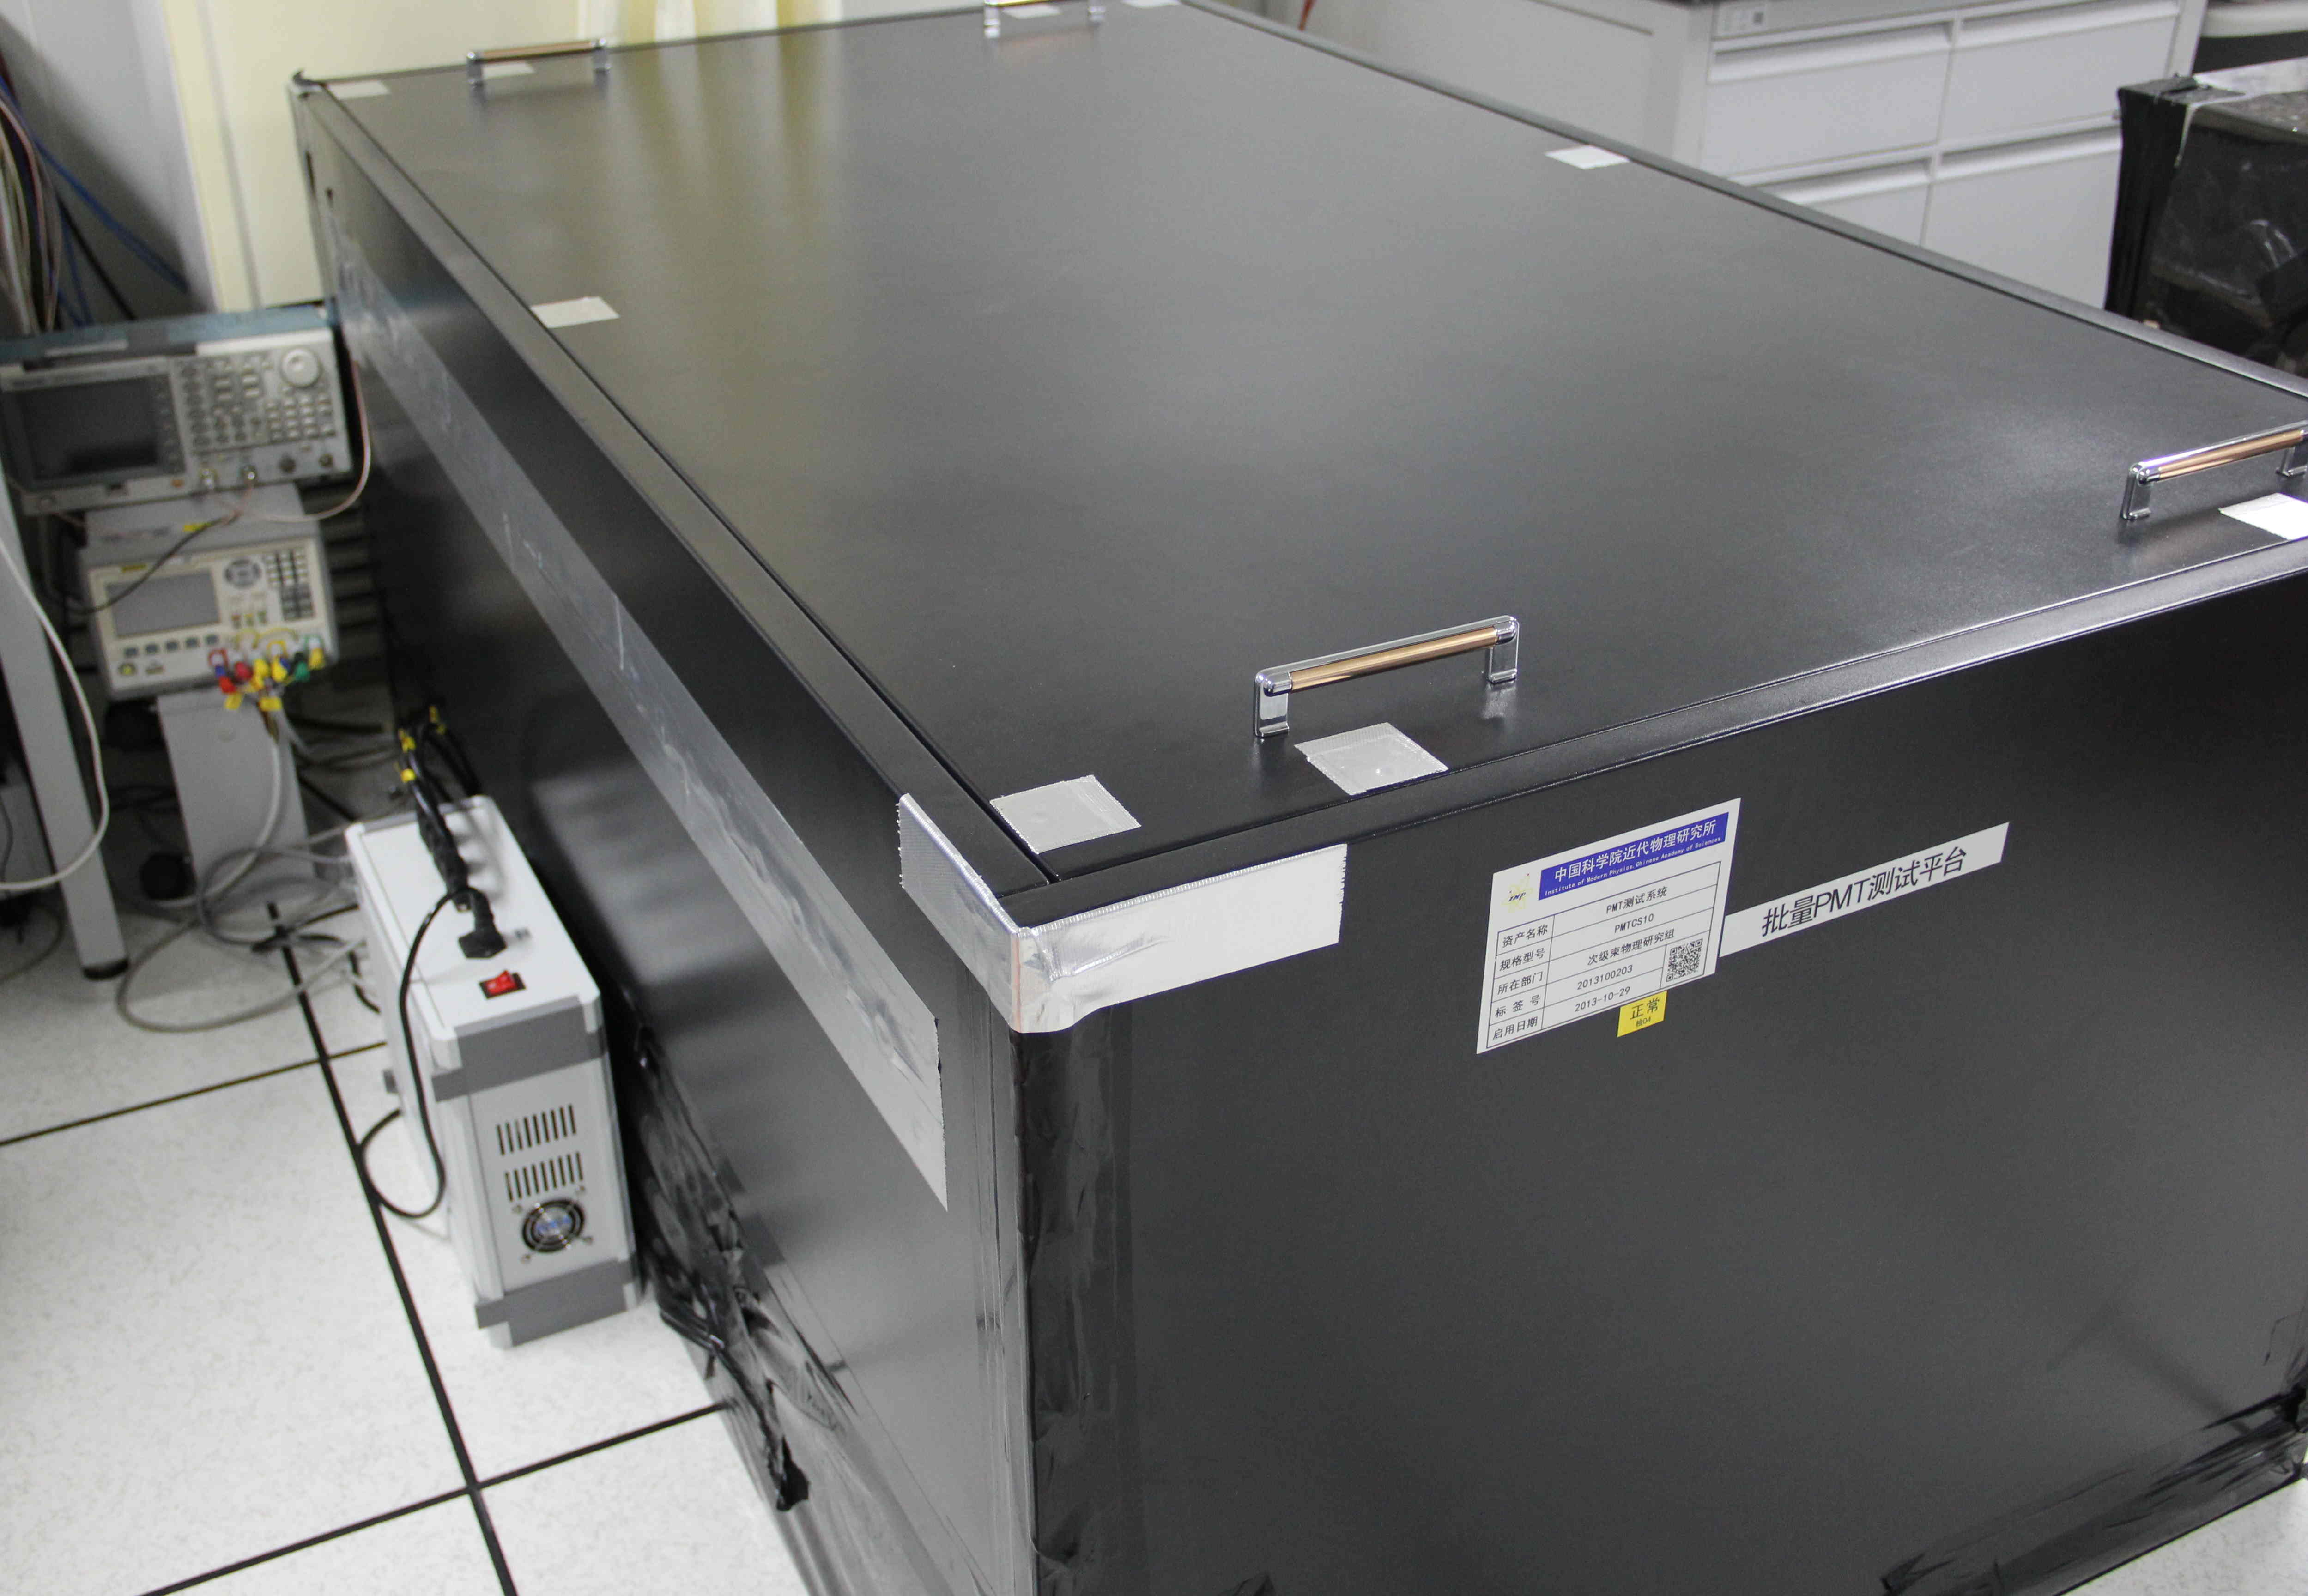
\includegraphics[width=0.49\textwidth]{chap/pmt_test/fig/black_box.jpg}
	}
	\subfloat[][三维移动平台与固定平台]{
		\label{fig:pmt_test:stages}
		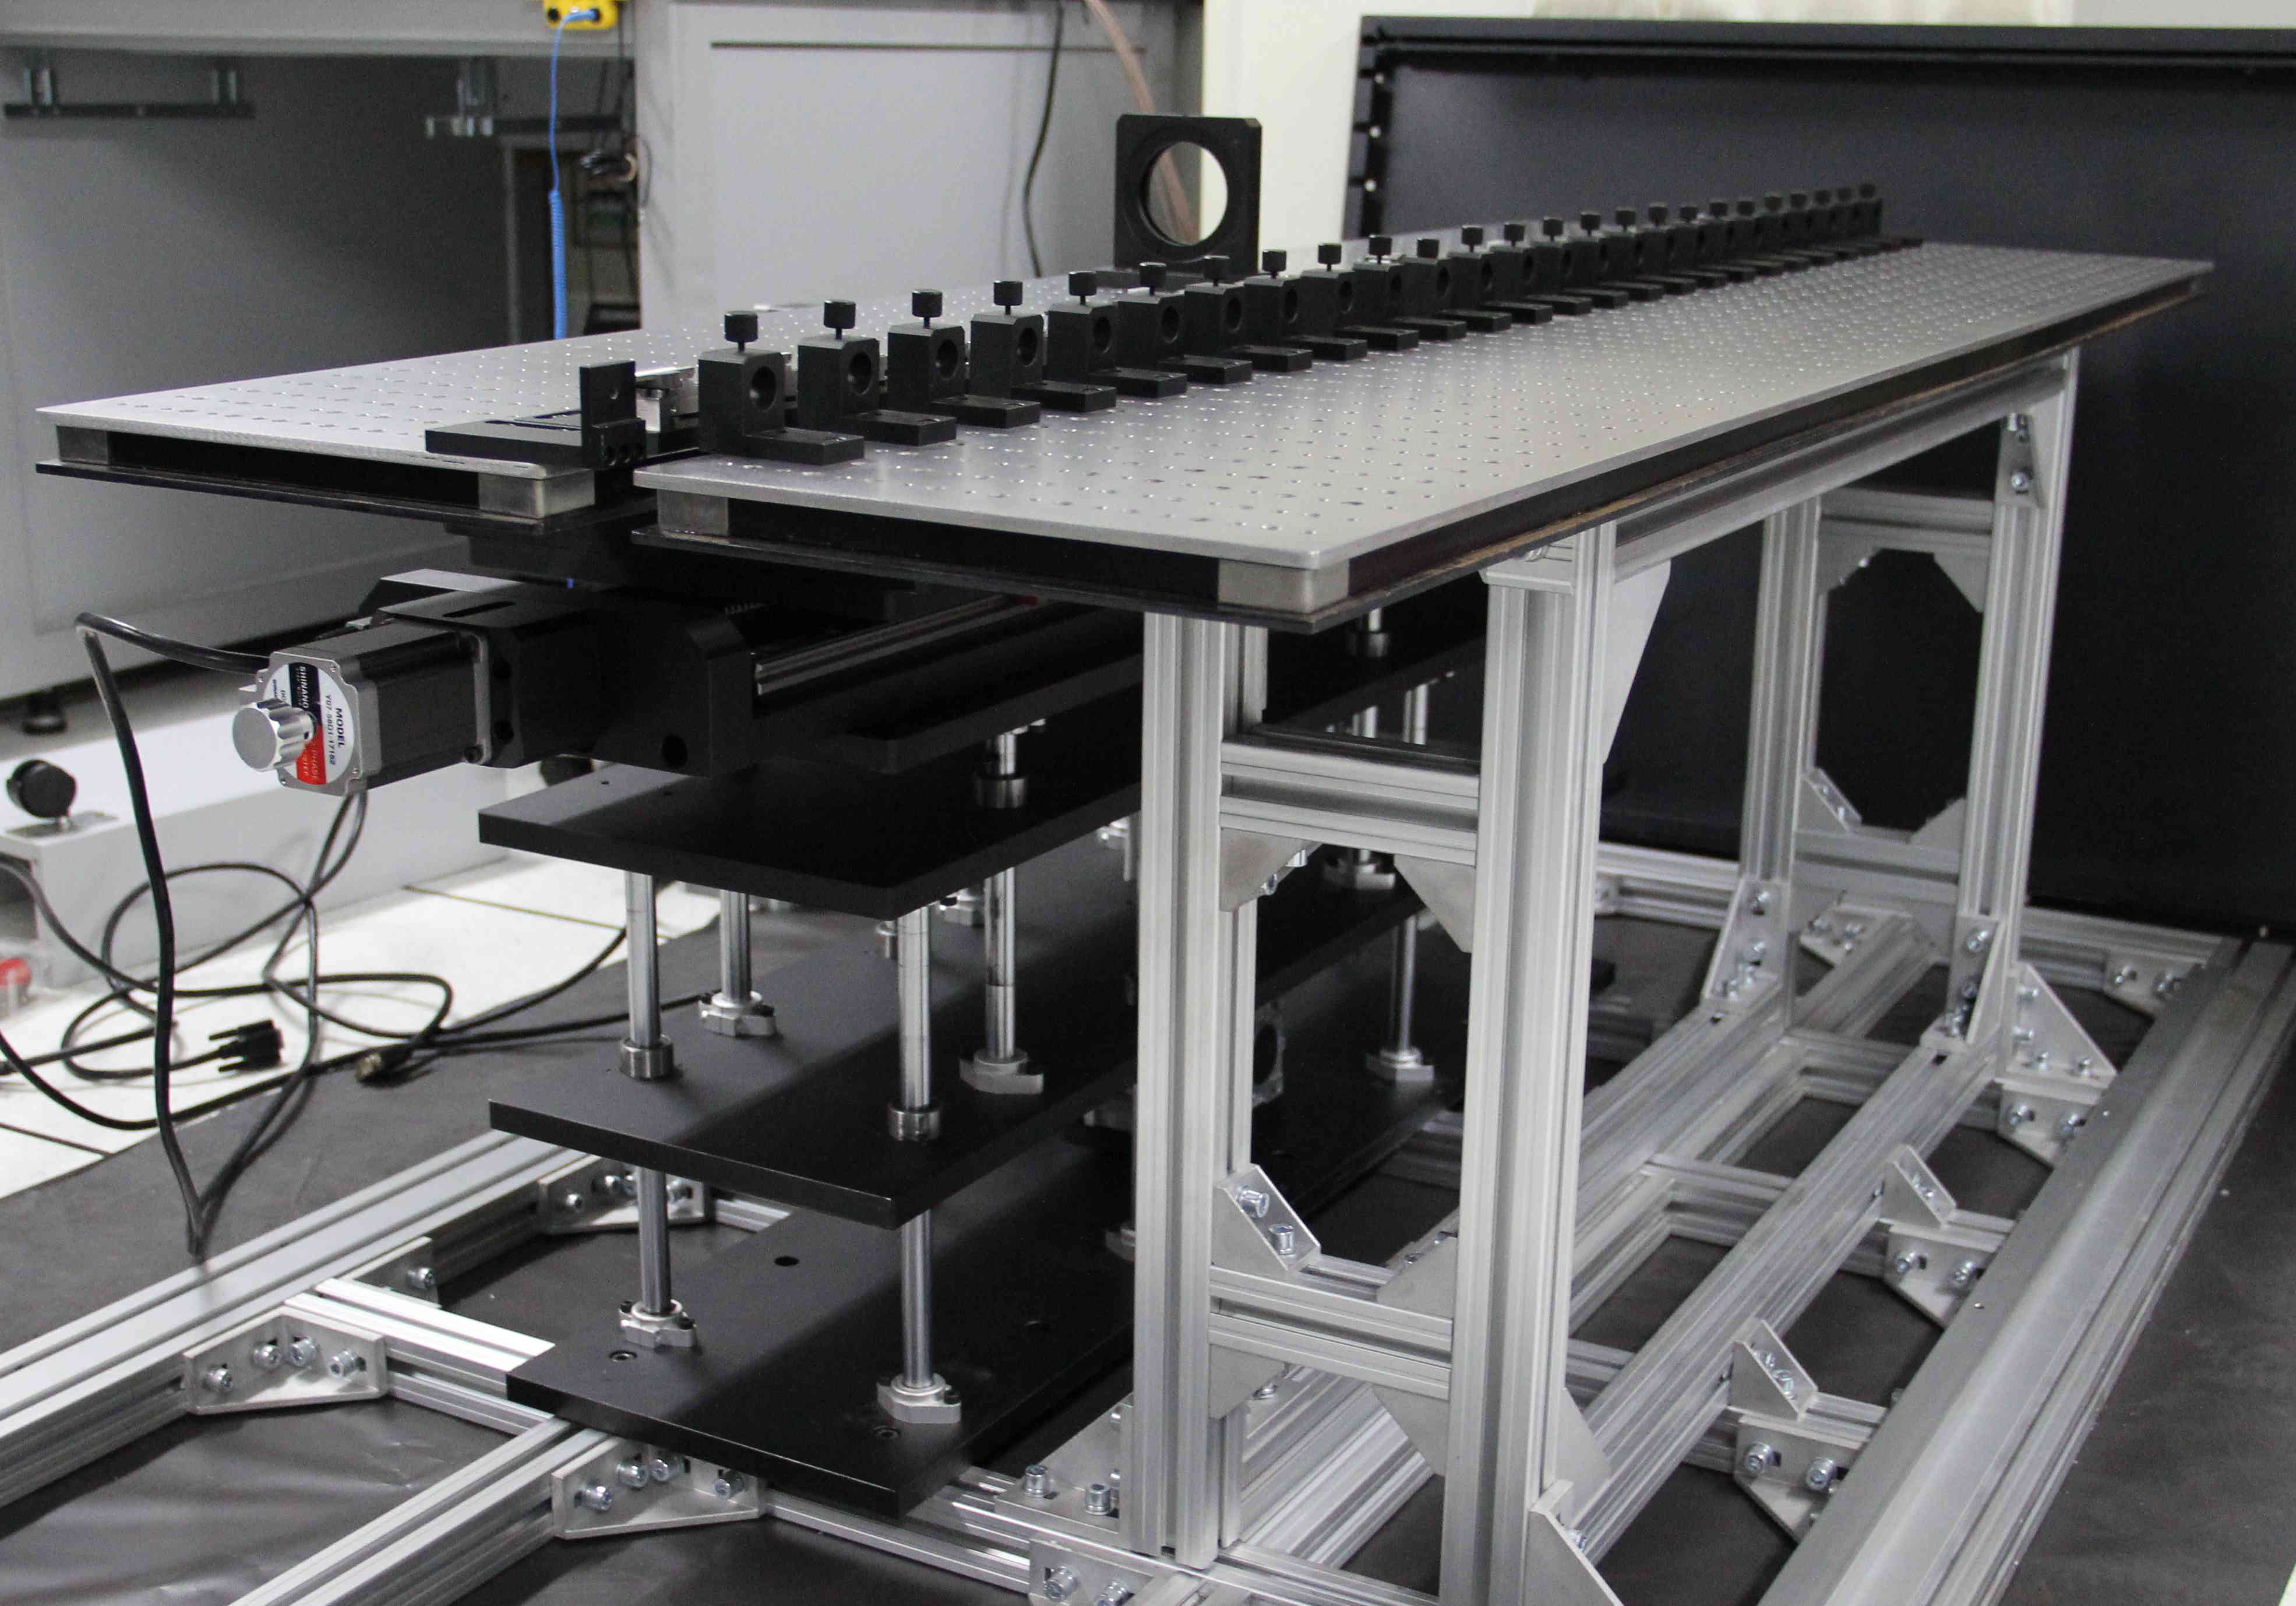
\includegraphics[width=0.49\textwidth]{chap/pmt_test/fig/stages.jpg}
	}
	\caption{PMT批量测试平台的主体结构}
	\label{fig:blindfigure}
\end{figure}

% 紧固件
\begin{figure}[htbp]
	\centering
	\includegraphics[width=0.6\textwidth]{chap/pmt_test/fig/fixtures.jpg}
	\caption{PMT紧固件和光纤紧固件}
	\label{fig:pmt_test:fixtures}
\end{figure}

% 光源
\begin{figure}[htbp]
	\centering
	\subfloat[][1)LED 2)积分球 3)集束光纤]{
		\label{fig:pmt_test:lightsource_components}
		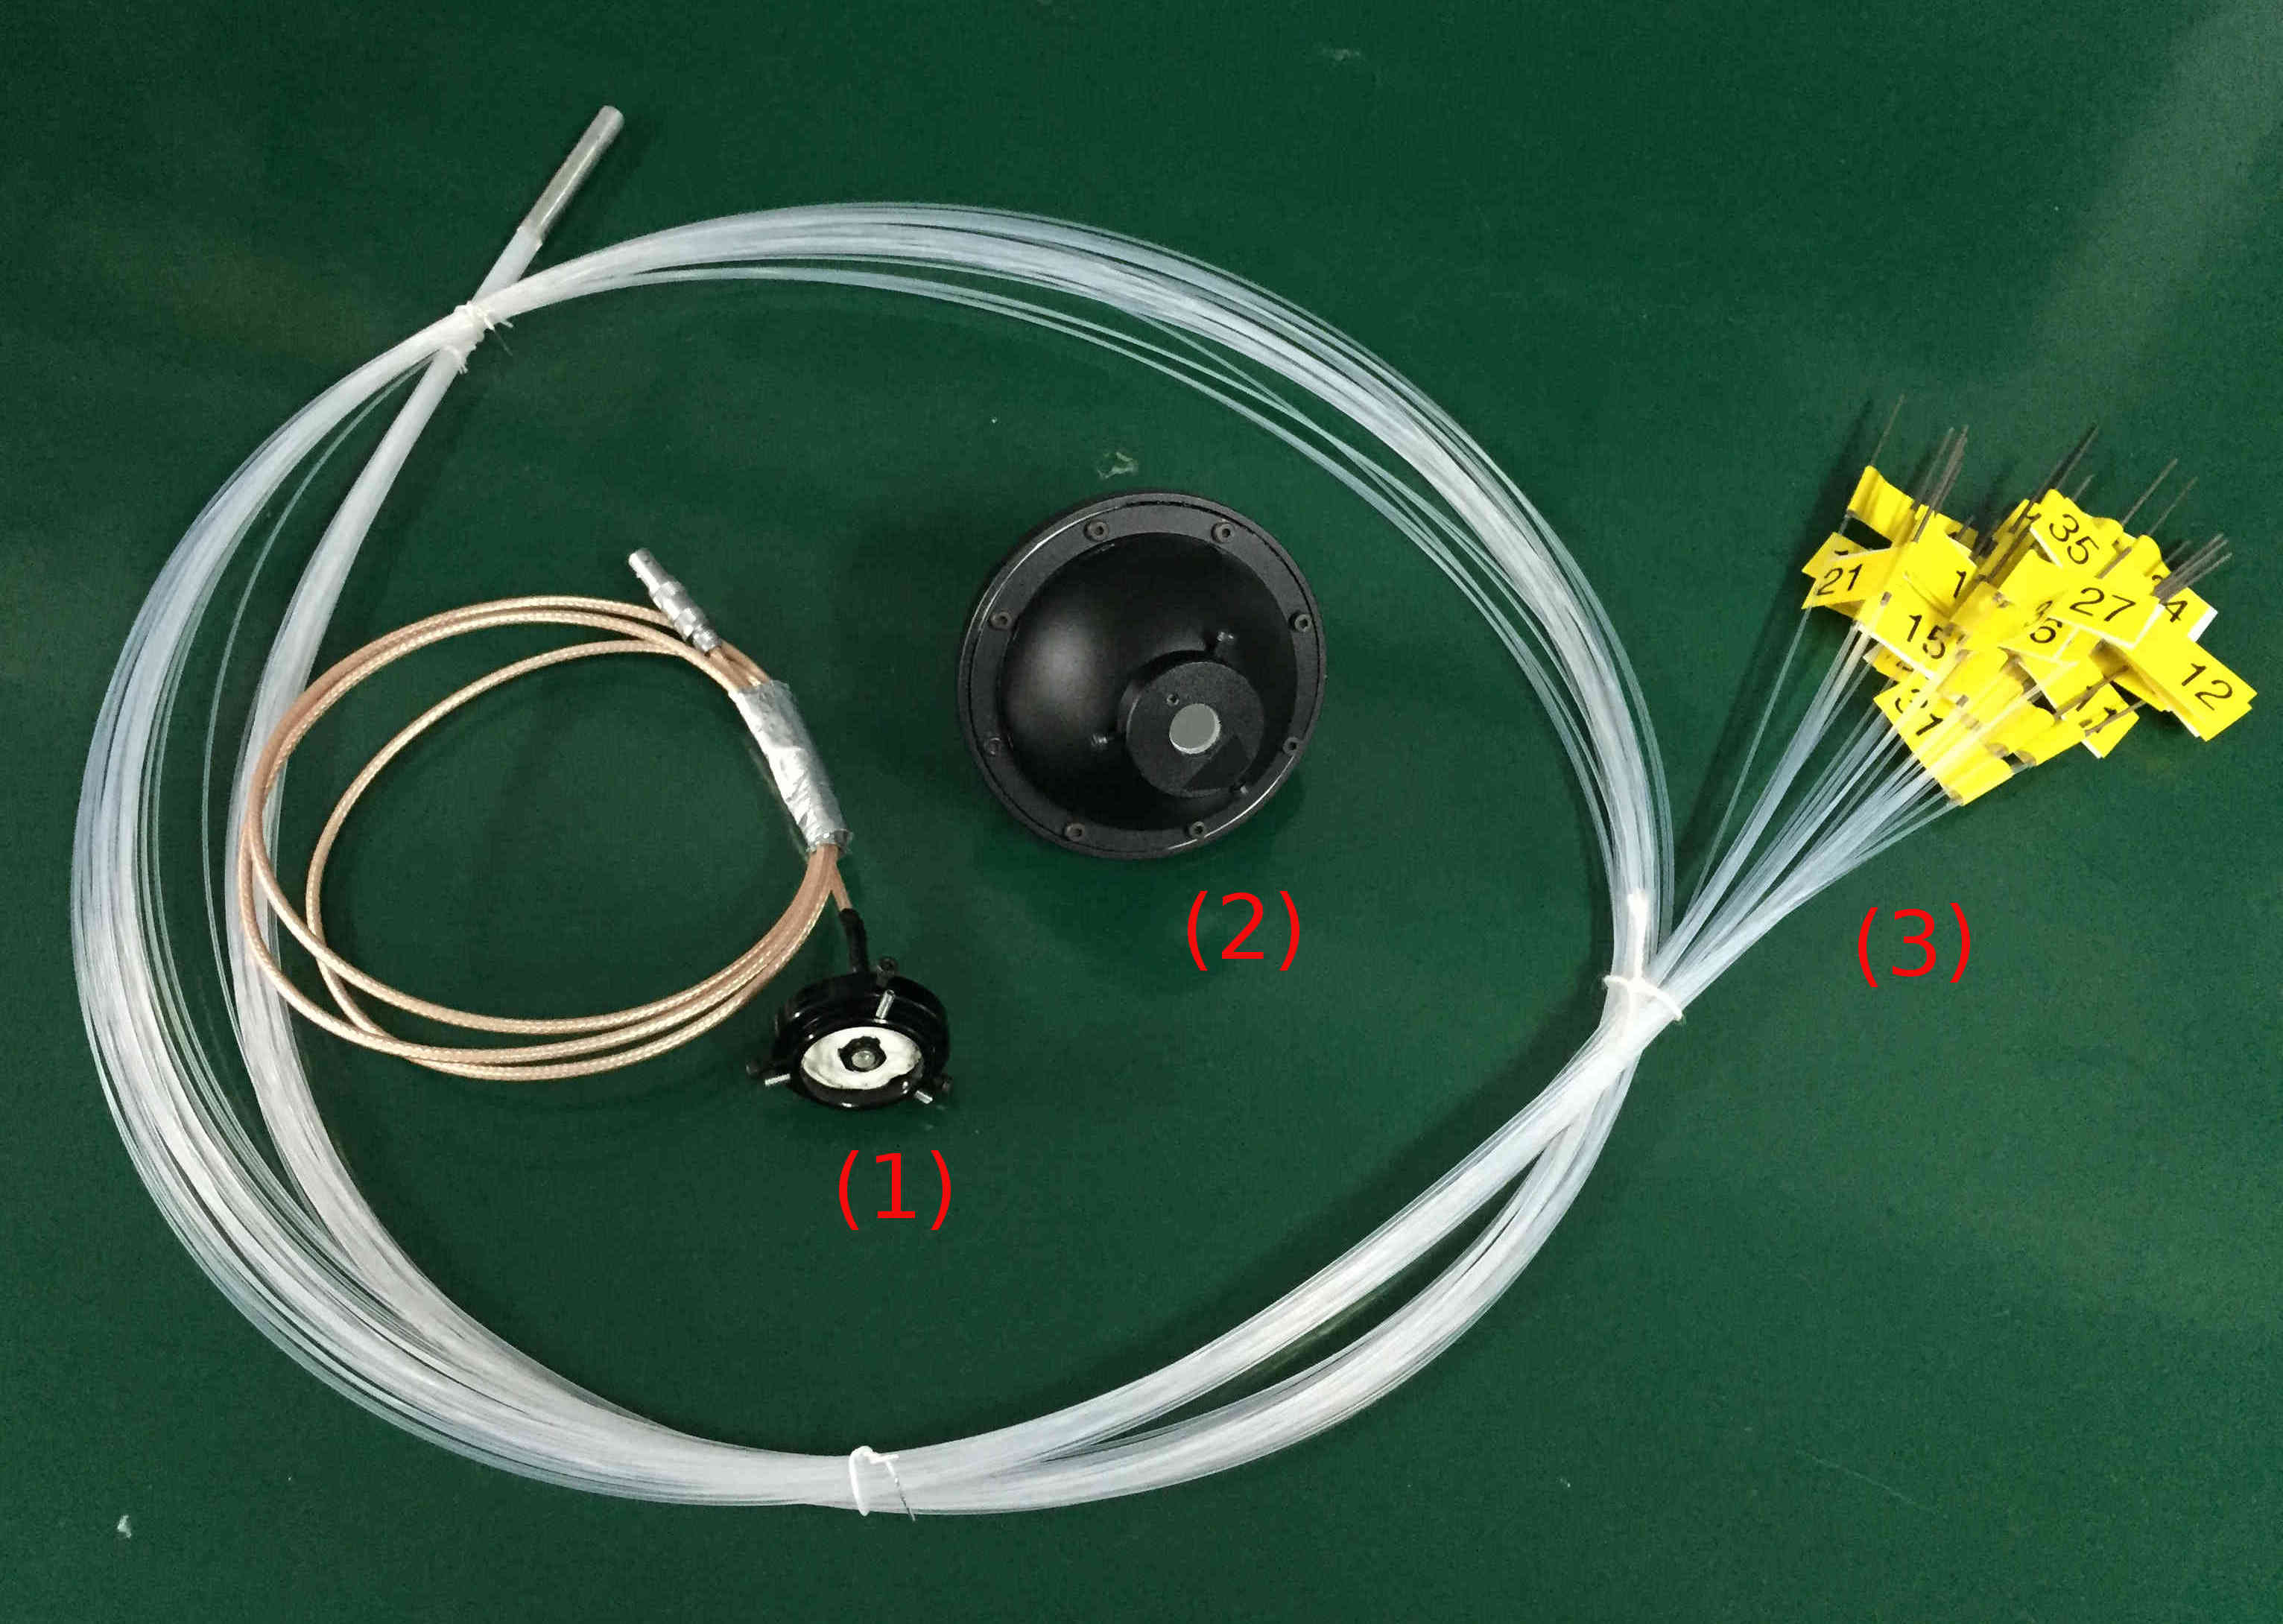
\includegraphics[width=0.49\textwidth]{chap/pmt_test/fig/lightsource_components.jpg}
	}
	\subfloat[][各组件耦合在一起]{
		\label{fig:pmt_test:lightsource_integration}
		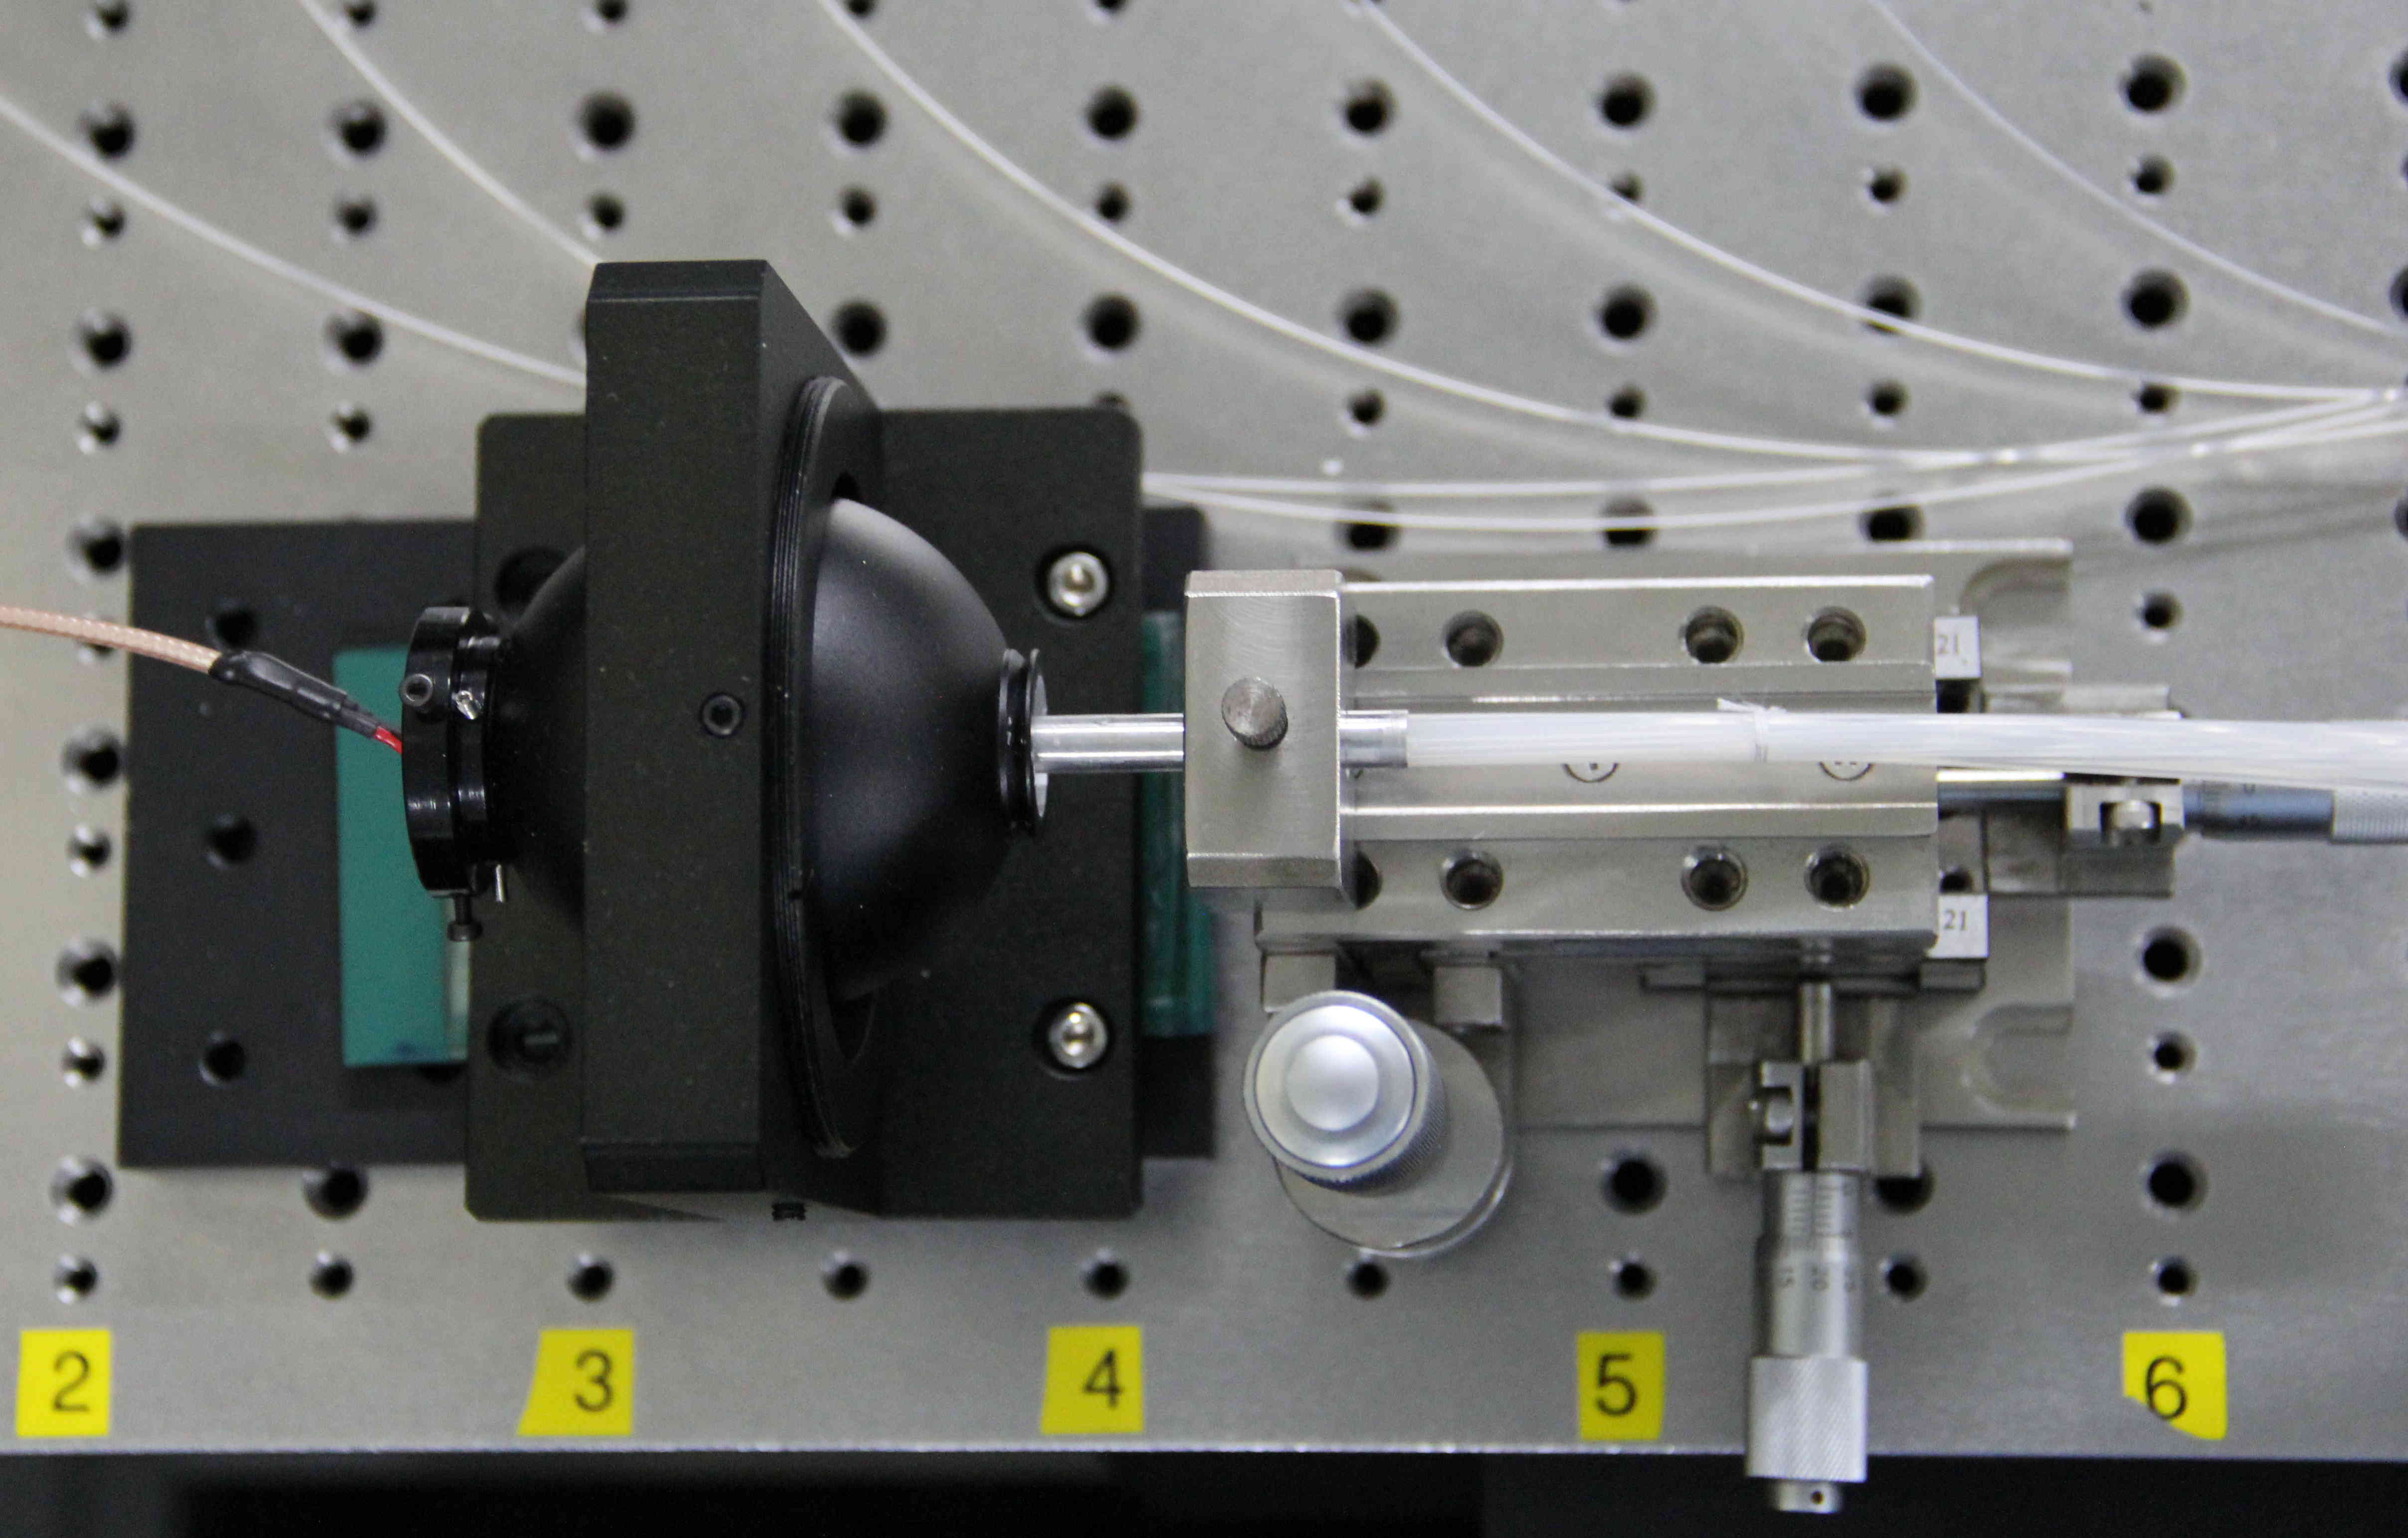
\includegraphics[width=0.49\textwidth]{chap/pmt_test/fig/lightsource_integration.jpg}
	}		
	\caption{PMT批量测试平台的光分配系统}
	\label{fig:pmt_test:light_distribution}
\end{figure}

\begin{figure}[htbp]
	\centering
	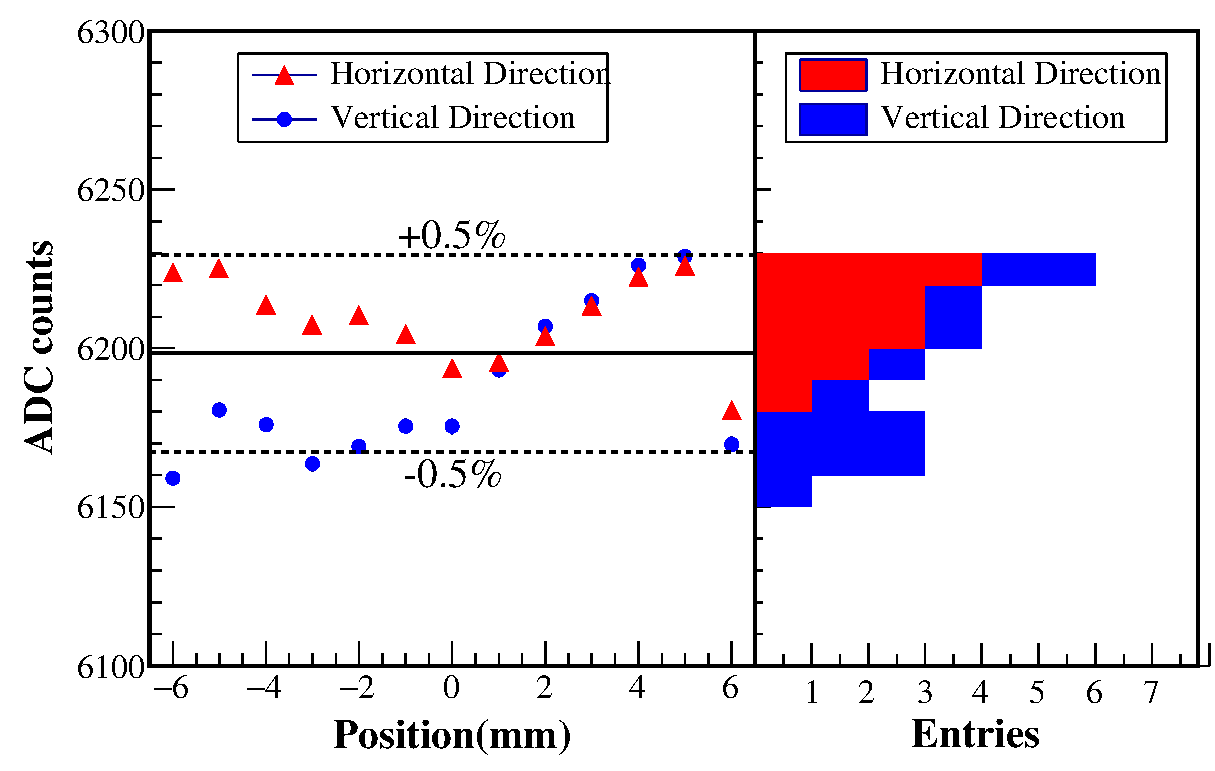
\includegraphics[width=0.65\textwidth]{chap/pmt_test/fig/integrationsphere_uniformity.eps}
	\caption{\SI{5}{cm}铝合金积分球输出端口的光均匀性}
	\label{fig:pmt_test:integrationsphere_uniformity}
\end{figure}

% 光源驱动器
\begin{figure}[htbp]
	\centering
	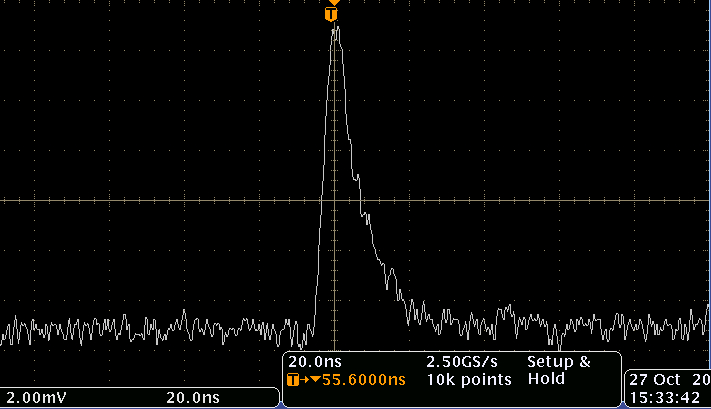
\includegraphics[width=0.65\textwidth]{chap/pmt_test/fig/led_pulse.jpg}
	\caption{输入方波脉冲驱动的LED光得到的R4443原始波形}
	\label{fig:pmt_test:led_pulse}
\end{figure}

\begin{figure}[htbp]
	\centering
	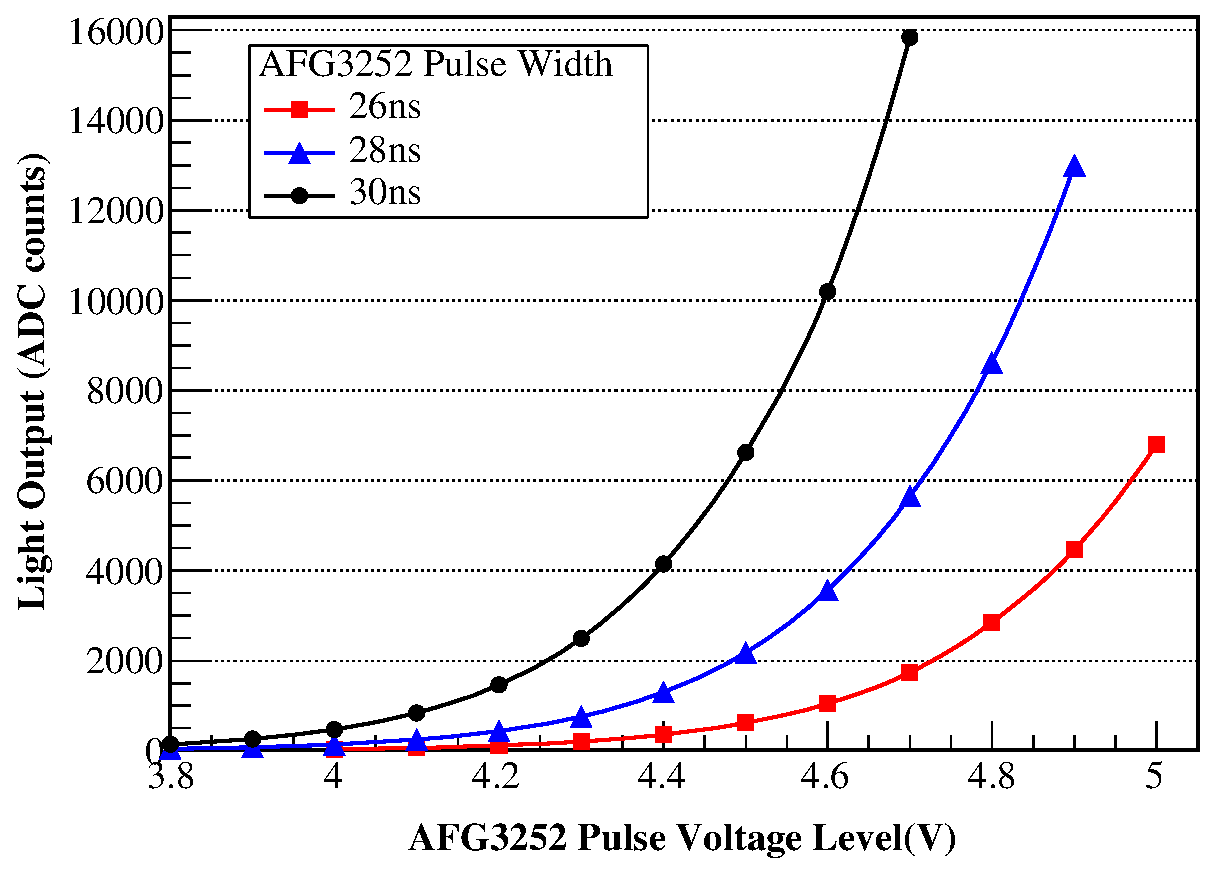
\includegraphics[width=0.62\textwidth]{chap/pmt_test/fig/led_response.eps}
	\caption{LED输出脉冲的光强度与AFG3253脉冲幅度的非线性关系}
	\label{fig:pmt_test:led_response}
\end{figure}

% 集束光纤
\begin{figure}[htbp]
	\centering
	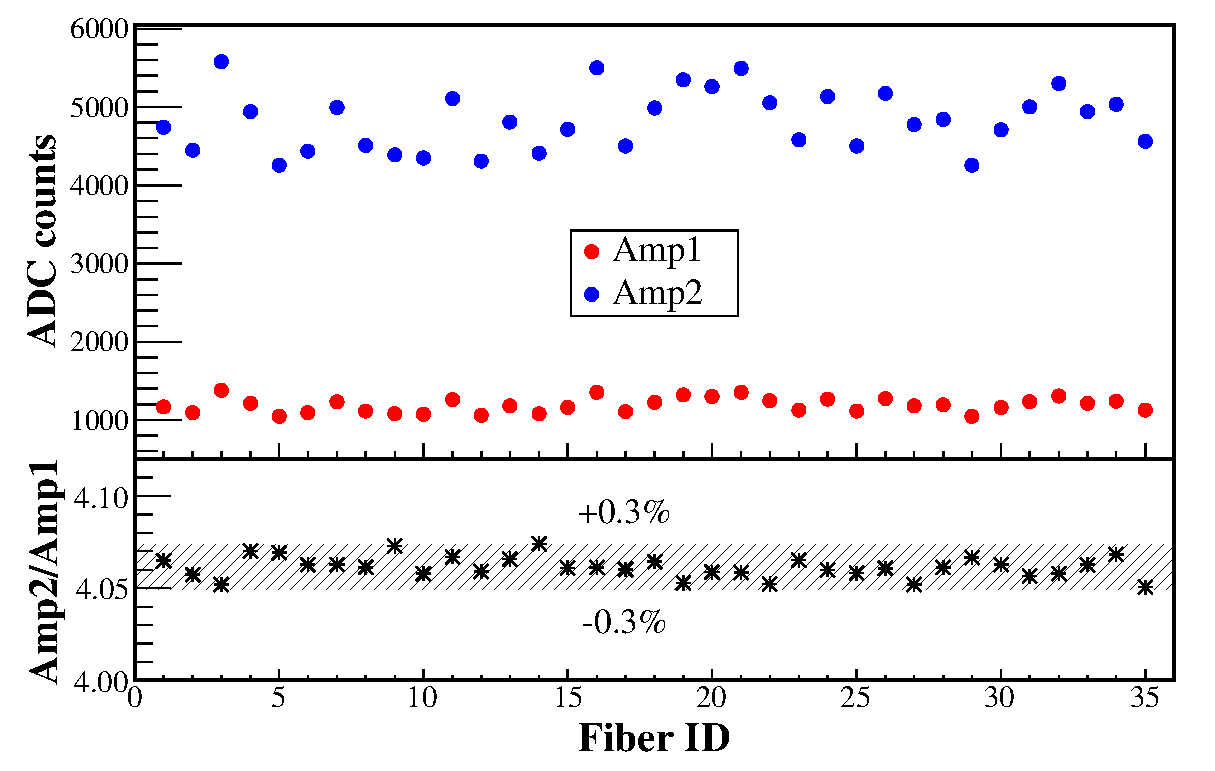
\includegraphics[width=0.7\textwidth]{chap/pmt_test/fig/fiber_difference.eps}
	\caption{集束光纤各通道的光传输差异性}
	\label{fig:pmt_test:fiber_difference}
\end{figure}

\subsection{测控软件}
% 最好这里做一个归纳性的介绍,具体细节设计放到附录中


\section{R4443裸管的性能测试}

\subsection{相对增益的测量}
\subsection{Dynode8/Dynode5增益比值的测量}
\subsection{光阴极均匀性}
\subsection{测试流程}

\section{PMT的筛选}
\subsection{筛选方案}
\subsection{参考单元模块的MIPs响应}
\subsection{与塑闪单元条的匹配}